%\documentclass{standalone}
%\usepackage{tikz}
%\usetikzlibrary{patterns,plotmarks}
%\begin{document}
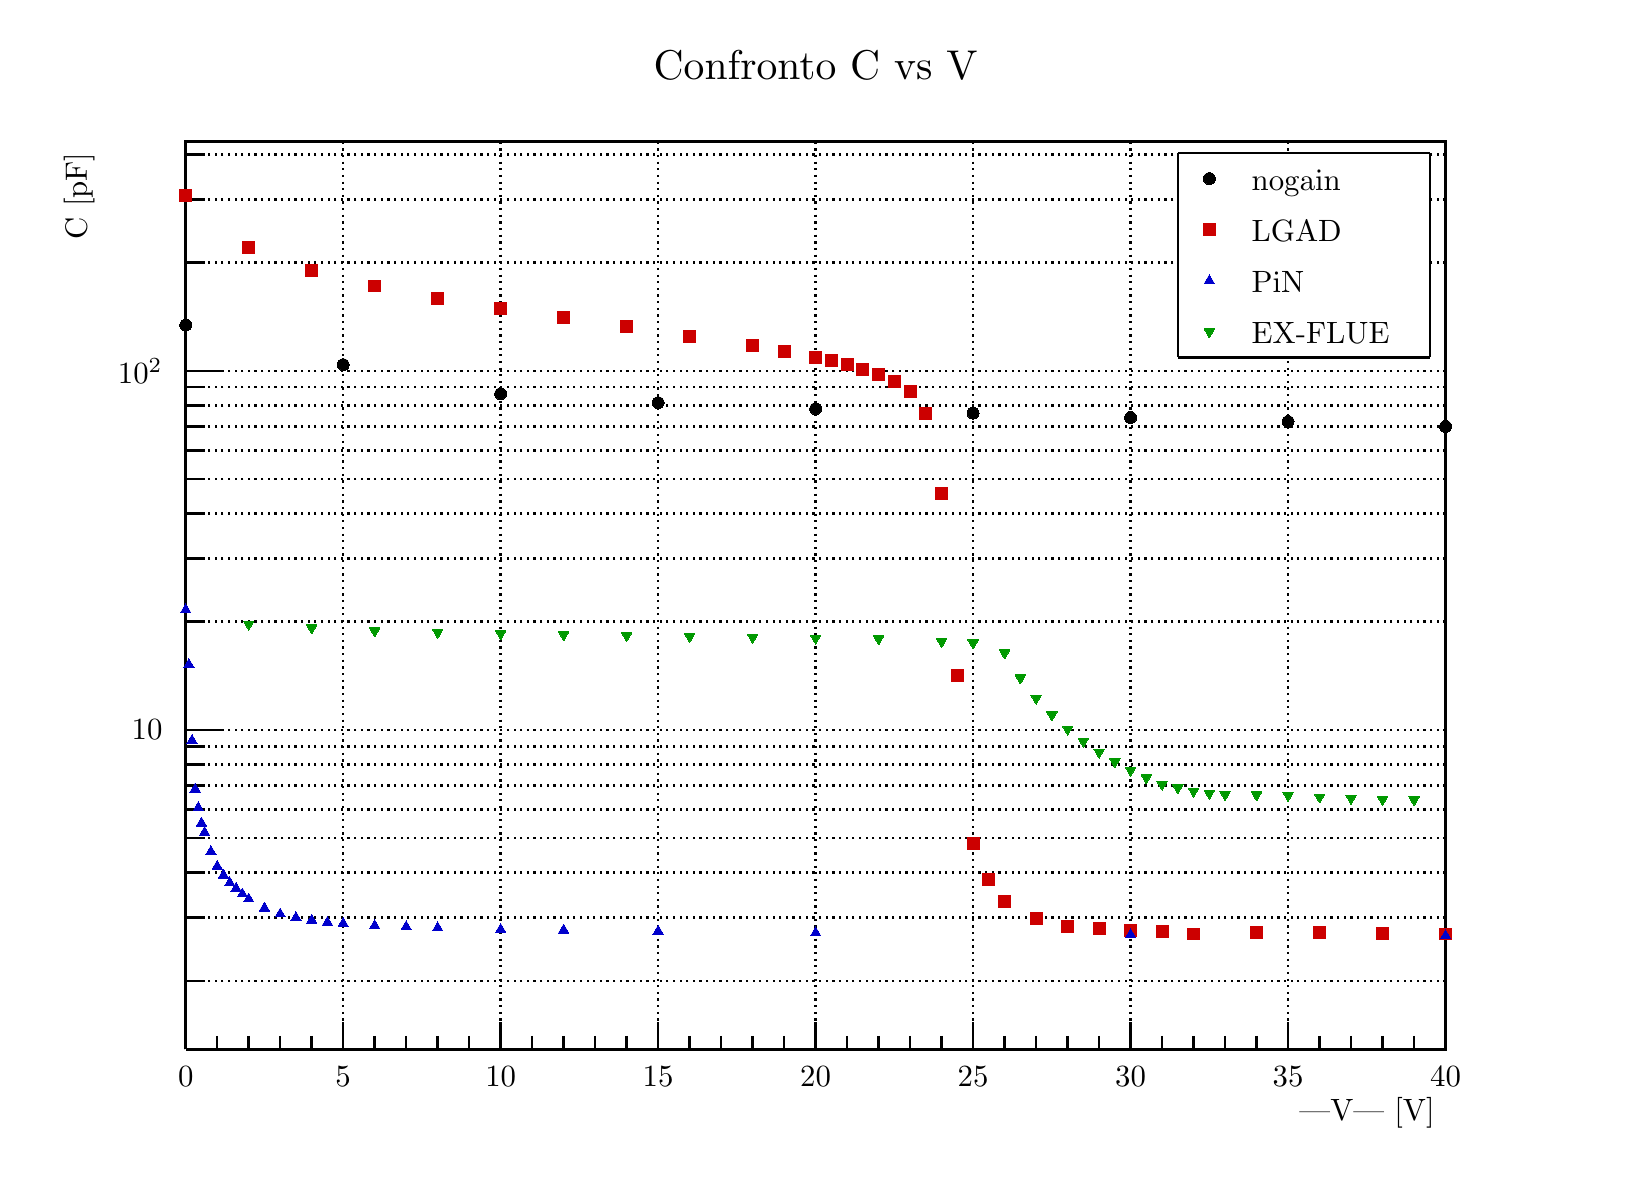
\begin{tikzpicture}
\def\CheckTikzLibraryLoaded#1{ \ifcsname tikz@library@#1@loaded\endcsname \else \PackageWarning{tikz}{usetikzlibrary{#1} is missing in the preamble.} \fi }
\CheckTikzLibraryLoaded{patterns}
\CheckTikzLibraryLoaded{plotmarks}
\pgfdeclareplotmark{cross} {
\pgfpathmoveto{\pgfpoint{-0.3\pgfplotmarksize}{\pgfplotmarksize}}
\pgfpathlineto{\pgfpoint{+0.3\pgfplotmarksize}{\pgfplotmarksize}}
\pgfpathlineto{\pgfpoint{+0.3\pgfplotmarksize}{0.3\pgfplotmarksize}}
\pgfpathlineto{\pgfpoint{+1\pgfplotmarksize}{0.3\pgfplotmarksize}}
\pgfpathlineto{\pgfpoint{+1\pgfplotmarksize}{-0.3\pgfplotmarksize}}
\pgfpathlineto{\pgfpoint{+0.3\pgfplotmarksize}{-0.3\pgfplotmarksize}}
\pgfpathlineto{\pgfpoint{+0.3\pgfplotmarksize}{-1.\pgfplotmarksize}}
\pgfpathlineto{\pgfpoint{-0.3\pgfplotmarksize}{-1.\pgfplotmarksize}}
\pgfpathlineto{\pgfpoint{-0.3\pgfplotmarksize}{-0.3\pgfplotmarksize}}
\pgfpathlineto{\pgfpoint{-1.\pgfplotmarksize}{-0.3\pgfplotmarksize}}
\pgfpathlineto{\pgfpoint{-1.\pgfplotmarksize}{0.3\pgfplotmarksize}}
\pgfpathlineto{\pgfpoint{-0.3\pgfplotmarksize}{0.3\pgfplotmarksize}}
\pgfpathclose
\pgfusepathqstroke
}
\pgfdeclareplotmark{cross*} {
\pgfpathmoveto{\pgfpoint{-0.3\pgfplotmarksize}{\pgfplotmarksize}}
\pgfpathlineto{\pgfpoint{+0.3\pgfplotmarksize}{\pgfplotmarksize}}
\pgfpathlineto{\pgfpoint{+0.3\pgfplotmarksize}{0.3\pgfplotmarksize}}
\pgfpathlineto{\pgfpoint{+1\pgfplotmarksize}{0.3\pgfplotmarksize}}
\pgfpathlineto{\pgfpoint{+1\pgfplotmarksize}{-0.3\pgfplotmarksize}}
\pgfpathlineto{\pgfpoint{+0.3\pgfplotmarksize}{-0.3\pgfplotmarksize}}
\pgfpathlineto{\pgfpoint{+0.3\pgfplotmarksize}{-1.\pgfplotmarksize}}
\pgfpathlineto{\pgfpoint{-0.3\pgfplotmarksize}{-1.\pgfplotmarksize}}
\pgfpathlineto{\pgfpoint{-0.3\pgfplotmarksize}{-0.3\pgfplotmarksize}}
\pgfpathlineto{\pgfpoint{-1.\pgfplotmarksize}{-0.3\pgfplotmarksize}}
\pgfpathlineto{\pgfpoint{-1.\pgfplotmarksize}{0.3\pgfplotmarksize}}
\pgfpathlineto{\pgfpoint{-0.3\pgfplotmarksize}{0.3\pgfplotmarksize}}
\pgfpathclose
\pgfusepathqfillstroke
}
\pgfdeclareplotmark{newstar} {
\pgfpathmoveto{\pgfqpoint{0pt}{\pgfplotmarksize}}
\pgfpathlineto{\pgfqpointpolar{44}{0.5\pgfplotmarksize}}
\pgfpathlineto{\pgfqpointpolar{18}{\pgfplotmarksize}}
\pgfpathlineto{\pgfqpointpolar{-20}{0.5\pgfplotmarksize}}
\pgfpathlineto{\pgfqpointpolar{-54}{\pgfplotmarksize}}
\pgfpathlineto{\pgfqpointpolar{-90}{0.5\pgfplotmarksize}}
\pgfpathlineto{\pgfqpointpolar{234}{\pgfplotmarksize}}
\pgfpathlineto{\pgfqpointpolar{198}{0.5\pgfplotmarksize}}
\pgfpathlineto{\pgfqpointpolar{162}{\pgfplotmarksize}}
\pgfpathlineto{\pgfqpointpolar{134}{0.5\pgfplotmarksize}}
\pgfpathclose
\pgfusepathqstroke
}
\pgfdeclareplotmark{newstar*} {
\pgfpathmoveto{\pgfqpoint{0pt}{\pgfplotmarksize}}
\pgfpathlineto{\pgfqpointpolar{44}{0.5\pgfplotmarksize}}
\pgfpathlineto{\pgfqpointpolar{18}{\pgfplotmarksize}}
\pgfpathlineto{\pgfqpointpolar{-20}{0.5\pgfplotmarksize}}
\pgfpathlineto{\pgfqpointpolar{-54}{\pgfplotmarksize}}
\pgfpathlineto{\pgfqpointpolar{-90}{0.5\pgfplotmarksize}}
\pgfpathlineto{\pgfqpointpolar{234}{\pgfplotmarksize}}
\pgfpathlineto{\pgfqpointpolar{198}{0.5\pgfplotmarksize}}
\pgfpathlineto{\pgfqpointpolar{162}{\pgfplotmarksize}}
\pgfpathlineto{\pgfqpointpolar{134}{0.5\pgfplotmarksize}}
\pgfpathclose
\pgfusepathqfillstroke
}
\definecolor{c}{rgb}{1,1,1};
\draw [color=c, fill=c] (0,0) rectangle (20,14.411);
\draw [color=c, fill=c] (2,1.4411) rectangle (18,12.9699);
\definecolor{c}{rgb}{0,0,0};
\draw [c,line width=0.9] (2,1.4411) -- (2,12.9699) -- (18,12.9699) -- (18,1.4411) -- (2,1.4411);
\definecolor{c}{rgb}{1,1,1};
\draw [color=c, fill=c] (2,1.4411) rectangle (18,12.9699);
\definecolor{c}{rgb}{0,0,0};
\draw [c,line width=0.9] (2,1.4411) -- (2,12.9699) -- (18,12.9699) -- (18,1.4411) -- (2,1.4411);
\draw [c,line width=0.9] (2,1.4411) -- (18,1.4411);
\draw [c,dash pattern=on 0.80pt off 1.60pt ,line width=0.9] (2,12.9699) -- (2,1.4411);
\draw [c,dash pattern=on 0.80pt off 1.60pt ,line width=0.9] (4,12.9699) -- (4,1.4411);
\draw [c,dash pattern=on 0.80pt off 1.60pt ,line width=0.9] (6,12.9699) -- (6,1.4411);
\draw [c,dash pattern=on 0.80pt off 1.60pt ,line width=0.9] (8,12.9699) -- (8,1.4411);
\draw [c,dash pattern=on 0.80pt off 1.60pt ,line width=0.9] (10,12.9699) -- (10,1.4411);
\draw [c,dash pattern=on 0.80pt off 1.60pt ,line width=0.9] (12,12.9699) -- (12,1.4411);
\draw [c,dash pattern=on 0.80pt off 1.60pt ,line width=0.9] (14,12.9699) -- (14,1.4411);
\draw [c,dash pattern=on 0.80pt off 1.60pt ,line width=0.9] (16,12.9699) -- (16,1.4411);
\draw [c,dash pattern=on 0.80pt off 1.60pt ,line width=0.9] (18,12.9699) -- (18,1.4411);
\draw [c,line width=0.9] (2,1.4411) -- (2,12.9699);
\draw [c,dash pattern=on 0.80pt off 1.60pt ,line width=0.9] (18,2.31307) -- (2,2.31307);
\draw [c,dash pattern=on 0.80pt off 1.60pt ,line width=0.9] (18,3.11608) -- (2,3.11608);
\draw [c,dash pattern=on 0.80pt off 1.60pt ,line width=0.9] (18,3.68582) -- (2,3.68582);
\draw [c,dash pattern=on 0.80pt off 1.60pt ,line width=0.9] (18,4.12775) -- (2,4.12775);
\draw [c,dash pattern=on 0.80pt off 1.60pt ,line width=0.9] (18,4.48883) -- (2,4.48883);
\draw [c,dash pattern=on 0.80pt off 1.60pt ,line width=0.9] (18,4.79412) -- (2,4.79412);
\draw [c,dash pattern=on 0.80pt off 1.60pt ,line width=0.9] (18,5.05857) -- (2,5.05857);
\draw [c,dash pattern=on 0.80pt off 1.60pt ,line width=0.9] (18,5.29184) -- (2,5.29184);
\draw [c,dash pattern=on 0.80pt off 1.60pt ,line width=0.9] (18,5.5005) -- (2,5.5005);
\draw [c,dash pattern=on 0.80pt off 1.60pt ,line width=0.9] (18,6.87325) -- (2,6.87325);
\draw [c,dash pattern=on 0.80pt off 1.60pt ,line width=0.9] (18,7.67626) -- (2,7.67626);
\draw [c,dash pattern=on 0.80pt off 1.60pt ,line width=0.9] (18,8.246) -- (2,8.246);
\draw [c,dash pattern=on 0.80pt off 1.60pt ,line width=0.9] (18,8.68793) -- (2,8.68793);
\draw [c,dash pattern=on 0.80pt off 1.60pt ,line width=0.9] (18,9.04901) -- (2,9.04901);
\draw [c,dash pattern=on 0.80pt off 1.60pt ,line width=0.9] (18,9.3543) -- (2,9.3543);
\draw [c,dash pattern=on 0.80pt off 1.60pt ,line width=0.9] (18,9.61875) -- (2,9.61875);
\draw [c,dash pattern=on 0.80pt off 1.60pt ,line width=0.9] (18,9.85202) -- (2,9.85202);
\draw [c,dash pattern=on 0.80pt off 1.60pt ,line width=0.9] (18,10.0607) -- (2,10.0607);
\draw [c,dash pattern=on 0.80pt off 1.60pt ,line width=0.9] (18,11.4334) -- (2,11.4334);
\draw [c,dash pattern=on 0.80pt off 1.60pt ,line width=0.9] (18,12.2364) -- (2,12.2364);
\draw [c,dash pattern=on 0.80pt off 1.60pt ,line width=0.9] (18,12.8062) -- (2,12.8062);
\draw [c,line width=0.9] (2,1.4411) -- (18,1.4411);
\draw [c,line width=0.9] (2,1.78697) -- (2,1.4411);
\draw [c,line width=0.9] (2.4,1.61404) -- (2.4,1.4411);
\draw [c,line width=0.9] (2.8,1.61404) -- (2.8,1.4411);
\draw [c,line width=0.9] (3.2,1.61404) -- (3.2,1.4411);
\draw [c,line width=0.9] (3.6,1.61404) -- (3.6,1.4411);
\draw [c,line width=0.9] (4,1.78697) -- (4,1.4411);
\draw [c,line width=0.9] (4.4,1.61404) -- (4.4,1.4411);
\draw [c,line width=0.9] (4.8,1.61404) -- (4.8,1.4411);
\draw [c,line width=0.9] (5.2,1.61404) -- (5.2,1.4411);
\draw [c,line width=0.9] (5.6,1.61404) -- (5.6,1.4411);
\draw [c,line width=0.9] (6,1.78697) -- (6,1.4411);
\draw [c,line width=0.9] (6.4,1.61404) -- (6.4,1.4411);
\draw [c,line width=0.9] (6.8,1.61404) -- (6.8,1.4411);
\draw [c,line width=0.9] (7.2,1.61404) -- (7.2,1.4411);
\draw [c,line width=0.9] (7.6,1.61404) -- (7.6,1.4411);
\draw [c,line width=0.9] (8,1.78697) -- (8,1.4411);
\draw [c,line width=0.9] (8.4,1.61404) -- (8.4,1.4411);
\draw [c,line width=0.9] (8.8,1.61404) -- (8.8,1.4411);
\draw [c,line width=0.9] (9.2,1.61404) -- (9.2,1.4411);
\draw [c,line width=0.9] (9.6,1.61404) -- (9.6,1.4411);
\draw [c,line width=0.9] (10,1.78697) -- (10,1.4411);
\draw [c,line width=0.9] (10.4,1.61404) -- (10.4,1.4411);
\draw [c,line width=0.9] (10.8,1.61404) -- (10.8,1.4411);
\draw [c,line width=0.9] (11.2,1.61404) -- (11.2,1.4411);
\draw [c,line width=0.9] (11.6,1.61404) -- (11.6,1.4411);
\draw [c,line width=0.9] (12,1.78697) -- (12,1.4411);
\draw [c,line width=0.9] (12.4,1.61404) -- (12.4,1.4411);
\draw [c,line width=0.9] (12.8,1.61404) -- (12.8,1.4411);
\draw [c,line width=0.9] (13.2,1.61404) -- (13.2,1.4411);
\draw [c,line width=0.9] (13.6,1.61404) -- (13.6,1.4411);
\draw [c,line width=0.9] (14,1.78697) -- (14,1.4411);
\draw [c,line width=0.9] (14.4,1.61404) -- (14.4,1.4411);
\draw [c,line width=0.9] (14.8,1.61404) -- (14.8,1.4411);
\draw [c,line width=0.9] (15.2,1.61404) -- (15.2,1.4411);
\draw [c,line width=0.9] (15.6,1.61404) -- (15.6,1.4411);
\draw [c,line width=0.9] (16,1.78697) -- (16,1.4411);
\draw [c,line width=0.9] (16.4,1.61404) -- (16.4,1.4411);
\draw [c,line width=0.9] (16.8,1.61404) -- (16.8,1.4411);
\draw [c,line width=0.9] (17.2,1.61404) -- (17.2,1.4411);
\draw [c,line width=0.9] (17.6,1.61404) -- (17.6,1.4411);
\draw [c,line width=0.9] (18,1.78697) -- (18,1.4411);
\draw [anchor=base] (2,0.965539) node[scale=1.11327, color=c, rotate=0]{0};
\draw [anchor=base] (4,0.965539) node[scale=1.11327, color=c, rotate=0]{5};
\draw [anchor=base] (6,0.965539) node[scale=1.11327, color=c, rotate=0]{10};
\draw [anchor=base] (8,0.965539) node[scale=1.11327, color=c, rotate=0]{15};
\draw [anchor=base] (10,0.965539) node[scale=1.11327, color=c, rotate=0]{20};
\draw [anchor=base] (12,0.965539) node[scale=1.11327, color=c, rotate=0]{25};
\draw [anchor=base] (14,0.965539) node[scale=1.11327, color=c, rotate=0]{30};
\draw [anchor=base] (16,0.965539) node[scale=1.11327, color=c, rotate=0]{35};
\draw [anchor=base] (18,0.965539) node[scale=1.11327, color=c, rotate=0]{40};
\draw [anchor= east] (18,0.634085) node[scale=1.11327, color=c, rotate=0]{|V| [V]};
\draw [c,line width=0.9] (2,1.4411) -- (2,12.9699);
\draw [c,line width=0.9] (2.24,2.31307) -- (2,2.31307);
\draw [c,line width=0.9] (2.24,3.11608) -- (2,3.11608);
\draw [c,line width=0.9] (2.24,3.68582) -- (2,3.68582);
\draw [c,line width=0.9] (2.24,4.12775) -- (2,4.12775);
\draw [c,line width=0.9] (2.24,4.48883) -- (2,4.48883);
\draw [c,line width=0.9] (2.24,4.79412) -- (2,4.79412);
\draw [c,line width=0.9] (2.24,5.05857) -- (2,5.05857);
\draw [c,line width=0.9] (2.24,5.29184) -- (2,5.29184);
\draw [c,line width=0.9] (2.48,5.5005) -- (2,5.5005);
\draw [anchor= east] (1.844,5.5005) node[scale=1.11327, color=c, rotate=0]{10};
\draw [c,line width=0.9] (2.24,6.87325) -- (2,6.87325);
\draw [c,line width=0.9] (2.24,7.67626) -- (2,7.67626);
\draw [c,line width=0.9] (2.24,8.246) -- (2,8.246);
\draw [c,line width=0.9] (2.24,8.68793) -- (2,8.68793);
\draw [c,line width=0.9] (2.24,9.04901) -- (2,9.04901);
\draw [c,line width=0.9] (2.24,9.3543) -- (2,9.3543);
\draw [c,line width=0.9] (2.24,9.61875) -- (2,9.61875);
\draw [c,line width=0.9] (2.24,9.85202) -- (2,9.85202);
\draw [c,line width=0.9] (2.48,10.0607) -- (2,10.0607);
\draw [anchor= east] (1.844,10.0607) node[scale=1.11327, color=c, rotate=0]{$10^{2}$};
\draw [c,line width=0.9] (2.24,11.4334) -- (2,11.4334);
\draw [c,line width=0.9] (2.24,12.2364) -- (2,12.2364);
\draw [c,line width=0.9] (2.24,12.8062) -- (2,12.8062);
\draw [anchor= east] (0.648371,12.9699) node[scale=1.11327, color=c, rotate=90]{C [pF]};
\foreach \P in {(2,10.6403), (4,10.1384), (6,9.76888), (8,9.65555), (10,9.57874), (12,9.52238), (14,9.46703), (16,9.41559), (18,9.3543)}{\draw[mark options={color=c,fill=c},mark size=2.162162pt, line width=0.000000pt, mark=*] plot coordinates {\P};}
\definecolor{c}{rgb}{0.8,0,0};
\foreach \P in {(2,12.2834), (2.8,11.6253), (3.6,11.333), (4.4,11.1373), (5.2,10.9834), (6,10.8504), (6.8,10.7312), (7.6,10.6167), (8.4,10.5015), (9.2,10.3777), (9.6,10.309), (10,10.2297), (10.2,10.1856), (10.4,10.1363), (10.6,10.0798),
 (10.8,10.0118), (11,9.92376), (11.2,9.7917), (11.4,9.51509), (11.6,8.50115), (11.8,6.19078), (12,4.05103), (12.2,3.59464), (12.4,3.31681), (12.8,3.10947), (13.2,3.00754), (13.6,2.97236), (14,2.95095), (14.4,2.93654), (14.8,2.90742), (15.6,2.92204),
 (16.4,2.92204), (17.2,2.91474), (18,2.90742)}{\draw[mark options={color=c,fill=c},mark size=2.162162pt, line width=0.000000pt, mark=square*] plot coordinates {\P};}
\definecolor{c}{rgb}{0,0,0.8};
\foreach \P in {(2,7.02567), (2.04,6.32974), (2.08,5.36528), (2.12,4.74833), (2.16,4.5118), (2.2,4.31651), (2.24,4.1978), (2.32,3.95399), (2.4,3.76826), (2.48,3.65589), (2.56,3.55801), (2.64,3.48813), (2.72,3.4157), (2.8,3.35228), (3,3.2377),
 (3.2,3.16176), (3.4,3.11608), (3.6,3.0828), (3.8,3.05576), (4,3.0421), (4.4,3.0145), (4.8,3.00055), (5.2,2.98651), (6,2.96525), (6.8,2.95811), (8,2.94376), (10,2.92204), (14,2.90007), (18,2.88529)}{\draw[mark options={color=c,fill=c},mark
 size=2.162162pt, line width=0.000000pt, mark=triangle*] plot coordinates {\P};}
\definecolor{c}{rgb}{0,0.6,0};
\foreach \P in {(2.8,6.84433), (3.6,6.79447), (4.4,6.75702), (5.2,6.73803), (6,6.72206), (6.8,6.7092), (7.6,6.69733), (8.4,6.68648), (9.2,6.67556), (10,6.66569), (10.8,6.65687), (11.6,6.62233), (12,6.60427), (12.4,6.47781), (12.6,6.15979),
 (12.8,5.90242), (13,5.68926), (13.2,5.51038), (13.4,5.35678), (13.6,5.21786), (13.8,5.09779), (14,4.98802), (14.2,4.89344), (14.4,4.81103), (14.6,4.76563), (14.8,4.7221), (15,4.69551), (15.2,4.68059), (15.6,4.67459), (16,4.66857), (16.4,4.64735),
 (16.8,4.63206), (17.2,4.61665), (17.6,4.61355)}{\draw[mark options={color=c,fill=c,rotate=180},mark size=2.162162pt, line width=0.000000pt, mark=triangle*] plot coordinates {\P};}
\definecolor{c}{rgb}{0,0,0};
\draw (10,13.9427) node[scale=1.50291, color=c, rotate=0]{Confronto C vs V};
\definecolor{c}{rgb}{1,1,1};
\draw [color=c, fill=c] (14.6,10.2318) rectangle (17.8,12.8258);
\definecolor{c}{rgb}{0,0,0};
\draw [c,line width=0.9] (14.6,10.2318) -- (17.8,10.2318);
\draw [c,line width=0.9] (17.8,10.2318) -- (17.8,12.8258);
\draw [c,line width=0.9] (17.8,12.8258) -- (14.6,12.8258);
\draw [c,line width=0.9] (14.6,12.8258) -- (14.6,10.2318);
\draw [anchor=base west] (15.4,12.3557) node[scale=1.11327, color=c, rotate=0]{nogain};
\foreach \P in {(15,12.5016)}{\draw[mark options={color=c,fill=c},mark size=2.162162pt, line width=0.000000pt, mark=*] plot coordinates {\P};}
\draw [anchor=base west] (15.4,11.7072) node[scale=1.11327, color=c, rotate=0]{LGAD};
\definecolor{c}{rgb}{0.8,0,0};
\foreach \P in {(15,11.8531)}{\draw[mark options={color=c,fill=c},mark size=2.162162pt, line width=0.000000pt, mark=square*] plot coordinates {\P};}
\definecolor{c}{rgb}{0,0,0};
\draw [anchor=base west] (15.4,11.0587) node[scale=1.11327, color=c, rotate=0]{PiN};
\definecolor{c}{rgb}{0,0,0.8};
\foreach \P in {(15,11.2046)}{\draw[mark options={color=c,fill=c},mark size=2.162162pt, line width=0.000000pt, mark=triangle*] plot coordinates {\P};}
\definecolor{c}{rgb}{0,0,0};
\draw [anchor=base west] (15.4,10.4102) node[scale=1.11327, color=c, rotate=0]{EX-FLUE};
\definecolor{c}{rgb}{0,0.6,0};
\foreach \P in {(15,10.5561)}{\draw[mark options={color=c,fill=c,rotate=180},mark size=2.162162pt, line width=0.000000pt, mark=triangle*] plot coordinates {\P};}
\end{tikzpicture}
%\end{document}
